\documentclass{article}
% translate with >> pdflatex -shell-escape <file>

% This file is used as unit test for pgfplots, copyright by Christian Feuersaenger.
% 
% See
%   http://pgfplots.sourceforge.net/pgfplots.pdf
% for pgfplots.
%
% Any required input files (for <plot table> or <plot file> or the table package) can be downloaded
% at
% http://www.ctan.org/tex-archive/graphics/pgf/contrib/pgfplots/doc/latex/
% and
% http://www.ctan.org/tex-archive/graphics/pgf/contrib/pgfplots/doc/latex/plotdata/

\usepackage{pgfplots}
\pgfplotsset{compat=newest}

\pagestyle{empty}

\begin{document}
\def\smallplotstest{%
	\addplot[smooth,blue,mark=*] coordinates {
		(-1,	1)
		(-0.75,	0.5625)
		(-0.5,	0.25)
		(-0.25,	0.0625)
		(0,		0)
		(0.25,	0.0625)
		(0.5,	0.25)
		(0.75,	0.5625)
		(1,		1)
	};
}
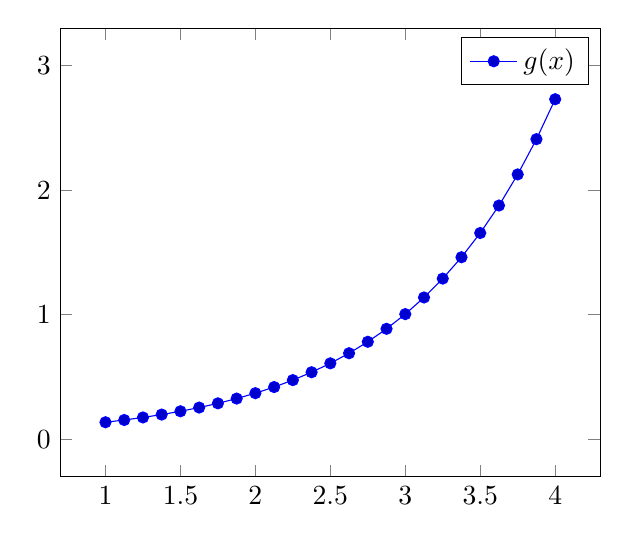
\begin{tikzpicture}
\begin{axis}[domain=1:4,ymin=0,ymax=3,enlargelimits]
\smallplotstest
\addlegendentry{$g(x)$}

\addplot (\x,{0.05*exp(\x)});
\addlegendentry{$f(x) = \frac{1}{20} \mathrm e^x$}
\end{axis}
\end{tikzpicture}
\end{document}
